
\includegraphics[height=1.25cm]{images/pictograms/elasticity}
\includegraphics[width=1.5cm]{images/pictograms/replication}

\lstinputlisting[language=bash,basicstyle=\small]{python_codes/fieldstone_63/keywords.ascii}

\par\noindent\rule{\textwidth}{0.4pt}

{\sl This stone was developed in collaboration with Taka Shinohara}.
\index{contributors}{Taka Shinohara}

\par\noindent\rule{\textwidth}{0.4pt}

%%%%%%%%%%%%%%%%%%%%%%%%%%%%%%%%%%%%%%%%%%%%%%%%%%%%%%%%%%%%%%%%%%%%%%%%%%%%%%%%%%%%%%%%

This \stone is based on \textcite{wowu95} (1995) published in Geophysical Research Letters. 
As for every \stone aiming at reproducing results off a publication I here include de abstract
of the article:

\begin{center}
\begin{minipage}{13cm}
{\small 
Grain crushing and pore collapse are important micromechanical processes responsible for hydrostatic and 
shear-enhanced compactions in porous rocks. These processes initiate from extensile microcracks which 
emanate from grain contacts. Microstructural observations indicate that such extensile cracking is inhibited 
in the vicinity of cemented grain contacts. The finite element technique was used to simulate the tensile 
stress concentration and normal stiffness in a cemented aggregate. The detrital grains were assumed to 
be elastically identical spheres bonded by cement layers of finite thickness. The numerical simulations 
show that the maximum tensile stress concentration is located near the triple junction (among grain, 
cement and pore space), and its magnitude is significantly less than that for an uncemented system. 
The development of microcracking near a cemented contact is readily inhibited unless the applied 
stress exceeds a critical value which is at least an order of magnitude greater than that for the 
onset of Hertzian fracture.
}
\end{minipage}
\end{center}

In this paper the authors use the finite element method to simulate 
the tensile stress concentration and normal stiffness in a cemented
aggregate. The grains are assumed to be elastically identical spheres
bonded by cement layers of finite thickness.

\begin{center}
\includegraphics[width=8cm]{python_codes/fieldstone_63/images/yoyo}
\includegraphics[width=6cm]{python_codes/fieldstone_63/images/domain}\\
{\captionfont Left: model of cemented granular system for 
axisymmetric finite element analysis (taken from \cite{wowu95}); Right: 
Domain for a\_fac=0.2 and h\_fac=5/90 and $R=90\mu m$.}
\end{center}

We define
\[
a_{fac} = \frac{a}{R}  
\qquad
\text{and}
\qquad 
h_{fac} = \frac{h}{R}
\]
which translates as follows in the code:
\begin{lstlisting}
outer_radius=90e-6      #radius R (m)  
a_fac = 20/90           # ratio of a to R 
h_fac = 5/90            # ratio of h to R
a = outer_radius*a_fac
h = outer_radius*h_fac
\end{lstlisting}

The material properties for the grain and the cement are as follows:

\begin{lstlisting}
#Quartz mechanical properties
E1 = 95e9                       # Young's modulus (Pa)
nu1=0.08                        # poisson ratio
mu1= E1/(2*(1+nu1))             # shear modulus
lambdaa1=2.*mu1*nu1/(1.-2.*nu1)  
\end{lstlisting}
and
\begin{lstlisting}
#cement mechanical properties 2 
E2 = 84e9                       # Young's modulus (Pa)
nu2=0.31                        # poisson ratio
mu2= E2/(2*(1+nu2))             # shear modulus
lambdaa2=2.*mu2*nu2/(1.-2.*nu2)  
\end{lstlisting}

Note that since gravitational effects are neglected we set $\vec{g}=\vec{0}$
so that density actually play no role in the model.

The mesh in the code is built in three phases: first, the quarter grain is meshed 
with triangles. Second, the cement block is meshed and shaped so as to follow the 
shape of the grain. Finally both meshes are merged together:

\begin{center}
\includegraphics[width=5.5cm]{python_codes/fieldstone_63/images/wowu95b}
\includegraphics[width=8cm]{python_codes/fieldstone_63/images/mesh}\\
{\captionfont Left: quadtree-based mesh used in \cite{wowu95}; 
Right: low resolution fieldstone mesh.}
\end{center}

Boundary conditions are as follows: $u=0$ is prescribed on the left and top boundary, 
while $v=0$ is prescribed on the bottom boundary, as shown below.
Additionally, traction b.c. are prescribed at the top\footnote{Note that 
in the axisymmetric case these then apply onto a disc and should be multiplied by $2\pi$} (these
are described in Section~\ref{MMM-ss:openbc}) as indicated hereunder:
\begin{center}
a)\includegraphics[width=5cm]{python_codes/fieldstone_63/images/bc_u}
b)\includegraphics[width=5cm]{python_codes/fieldstone_63/images/bc_v}\\
c)\includegraphics[width=4cm]{python_codes/fieldstone_63/images/wowu95}\\
{\captionfont a,b) Horizontal and vertical displacement boundary condition indicator.
c) Imposed traction at the top surface (Taken from \cite{wowu95}).}
\end{center}

Linear triangular elements are used and a 3-point numerical quadrature is used.
Average elemental quantities are computed with 7 quadrature points.
These same quantities are also projected onto the nodes for visualisation purposes.
Principal stresses are computed as explained in Section~\ref{MMM-sec:princ_stress}.

The code solves the FE system and retrieves the deformation components $x$ and $y$,
or $r$ and $z$ in the axisymmetric case.
Average elemental strain components are then computed. In the axisymmetric case
then  $\varepsilon_{\theta\theta}$ is computed and otherwise set to zero in the plane strain case.
The stress tensor components are then computed as follows:
\begin{eqnarray}
\sigma_{xx} &=& \lambda \vec\nabla\cdot\vec{u} + 2\mu \varepsilon_{xx} \\
\sigma_{zz} &=& \lambda \vec\nabla\cdot\vec{u} + 2\mu \varepsilon_{zz} \\
\sigma_{xz} &=&  2\mu \varepsilon_{xz} 
\end{eqnarray}
where $\vec\nabla\cdot\vec{u}=\frac{\partial u}{\partial x} + \frac{\partial w}{\partial z}$
in plane strain and 
$\vec\nabla\cdot\vec{u}=\frac{\partial u}{\partial x} + \frac{u}{x} + \frac{\partial w}{\partial z}$
in the axisymmetric case\footnote{Remember that the $xz$ plane is in fact the $rz$ plane so that 
the term $u_r/r$ becomes $u/x$ in practice.}.

Principal stresses are such that $\sigma_1>\sigma_2$ and 
\[
\sigma_{1,2}=\frac{\sigma_{xx}+\sigma_{yy}}{2} 
\pm \sqrt{  \left(\frac{\sigma_{xx}-\sigma_{yy}}{2}\right)^2 +\sigma_{xy}^2 }
 \]
The principal direction angle $\theta_p$ defines the principal
directions where the only stresses are normal stresses, and 
is given by the relationship:
\[
\tan (2\theta_p) =  \frac{2 \sigma_{xy}}{\sigma_{xx} -\sigma_{yy}}
\]
We find that $\theta_2$ is always negative, while $\theta_1$ showcases positive and negative values. 
We define the tensile zone as $\sigma_1>0$.

In general $\sigma_1$ is the maximum (most tensile) principal stress, 
$\sigma_3$ is the minimum (most compressive) principal stress, 
and $\sigma_2$ is the intermediate principal stress.

The maximum shear stress (in 2D) is given by
\[
\tau_{max} = \frac12(\sigma_1-\sigma_2)
\]

In the axisymmetric case the stress tensor is given by 
\[
{\bm \sigma} = 
\left(
\begin{array}{ccc}
\sigma_{rr} & 0 & \sigma_{rz} \\
0 & \sigma_{\theta\theta} & 0 \\
\sigma_{rz} & 0 & \sigma_{zz} 
\end{array}
\right)
\]
There are now three eigenvalues. However it is obvious that $\sigma_{\theta\theta}$ is 
one of them and the other two correspond to those of the $2\times 2$ stress stensor with 
$\sigma_{rr}$, $\sigma_{rz}$ and $\sigma_{zz}$ terms.
The code therefore needs not be modified to compute these. 



\begin{center}
\includegraphics[width=8.5cm]{python_codes/fieldstone_63/images/wowu95c}\\
{\captionfont Contours for the minimum principal stress in the vicinity of the triple junction}
\end{center}

\begin{remark}
This paper by Wong and Wu is a nice example of not-reproducible science. For one, boundary conditions 
are not all specified. Second, it is not specified whether the results are obtained in plane strain 
or axisymmetric geometry. Third, the program that was used is proprietary (ABAQUS). 
Fourth, no resolution tests are presented: given how small the area A is, and how comparable 
in size it is to the elements, this is problematic. Fifth, it is not clear how the 
tensile zone is defined. Sixth: the type of finite element is not specified. Seven, 
we are shown one field which is a derivative of the solution (displacement) but not the 
solution itelf.  
\end{remark}

The following results are obtained with very high resolutions, i.e. 
nLayers=901, nel\_h=80. This yields a mesh with about 1.6M triangles, 
and Nfem=1,668,488.

\newpage
%-----------------------------------------------------------------------
\paragraph{Results in plane strain}


\begin{center}
\includegraphics[width=5.5cm]{python_codes/fieldstone_63/results/ps/disp}
\includegraphics[width=5.5cm]{python_codes/fieldstone_63/results/ps/disp_x}
\includegraphics[width=5.5cm]{python_codes/fieldstone_63/results/ps/disp_y}\\
\includegraphics[width=5.5cm]{python_codes/fieldstone_63/results/ps/sigma1}
\includegraphics[width=5.5cm]{python_codes/fieldstone_63/results/ps/sigma2}
\includegraphics[width=5.5cm]{python_codes/fieldstone_63/results/ps/strain}\\
\includegraphics[width=5.5cm]{python_codes/fieldstone_63/results/ps/angle}
\includegraphics[width=5.5cm]{python_codes/fieldstone_63/results/ps/maximum_shear_stress}
\includegraphics[width=5.5cm]{python_codes/fieldstone_63/results/ps/tensile}
\end{center}

\newpage
%-----------------------------------------------------------------------
\paragraph{Results in axisymmetric geometry}

\begin{center}
\includegraphics[width=5.5cm]{python_codes/fieldstone_63/results/axi/disp}
\includegraphics[width=5.5cm]{python_codes/fieldstone_63/results/axi/disp_x}
\includegraphics[width=5.5cm]{python_codes/fieldstone_63/results/axi/disp_y}\\
\includegraphics[width=5.5cm]{python_codes/fieldstone_63/results/axi/sigma1}
\includegraphics[width=5.5cm]{python_codes/fieldstone_63/results/axi/sigma2}
\includegraphics[width=5.5cm]{python_codes/fieldstone_63/results/axi/strain}\\
\includegraphics[width=5.5cm]{python_codes/fieldstone_63/results/axi/angle}
\includegraphics[width=5.5cm]{python_codes/fieldstone_63/results/axi/maximum_shear_stress}
\includegraphics[width=5.5cm]{python_codes/fieldstone_63/results/axi/tensile}
\end{center}

